%%=============================================================================
%% Resultaten
%%=============================================================================

\chapter{Resultaten}
\label{ch:resultaten}

\section{Vergelijking verschillende technieken}
\label{sec:technieken}

%% TODO:
%% Uit je probleemstelling moet duidelijk zijn dat je onderzoek een meerwaarde
%% heeft voor een concrete doelgroep (bv. een bedrijf).
%%
%% Wees zo concreet mogelijk bij het formuleren van je
%% onderzoeksvra(a)g(en). Een onderzoeksvraag is trouwens iets waar nog
%% niemand op dit moment een antwoord heeft (voor zover je kan nagaan).
Verschillende van de voorgestelde technieken worden reeds automatisch toegepast door Android Studio bij het compileren van de applicatie. Zo zit Proguard ingebouwd in Android Studio, worden ongebruikte resources verwijderd door de ingebouwde lint tool en kunnen enumeraties automatisch omgezet worden naar integers. Hierdoor zal het handmatig uitvoeren van deze technieken geen extra effect teweeg brengen. Daarnaast zal het effect van de technieken afhankelijk zijn van het app-profiel. 
Legende technieken: 
\begin{enumerate}
	\setcounter{enumi}{-1}
	\item Techniek0 = Geen compressietechniek toegepast
	\item Techniek1 = Verwijder ongebruikte resources
	\item Techniek2 = Comprimeer afbeeldingen
	\item Techniek3 = Gebruik WebP-formaat
	\item Techniek4 = Verklein grootte native binaries
\end{enumerate}
\subsection{Foto-app}
Bij de eerste applicatie die getest werd, een foto-app die veel mediabestanden bevat, had vooral het gebruik van het WebP-formaat voor alle afbeeldingen een grote invloed op de grootte van de APK. De afbeeldingen werden omgezet van het PNG-formaat naar het WebP-formaat met lossless compressie, waardoor er dus niet in kwaliteit van de afbeeldinge ingeboet moet worden. Door het toepassen van deze compressietechniek werd de grootte van de APK meer dan vervierdubbeld. In de gedetailleerde analyse van de APK in Android Studio kon waargenomen worden dat vooral de res/ folder, die de afbeeldingen die in de app gebruikt worden bevat, al de extra opslagruimte die werd ingenomen inneemt. Dit is een onverwacht resultaat, aangezien er door Google wordt aangeraden om deze techniek te gebruiken om de grootte van de APK te verkleinen. De andere technieken brachten op dit vlak geen verandering. Op vlak van het geheugengebruik van de applicatie tijdens runtime kon een minieme verandering van 0.03MB meer geheugen gebruikt opgemerkt worden na het toepassen van de techniek ``Verklein resource gebruik van libraries``. Na de omzetting van de afbeeldingen naar het WebP-formaat verhoogde het CPU-gebruik met 9 procent. Dit wordt veroorzaakt doordat het genereren van de WebP-afbeeldingen meer CPU-kracht vergt.
\begin{figure}[H]
	\centering
	\caption{\textit{Resultaten verschillende compressietechnieken op APK-grootte foto-app}}
	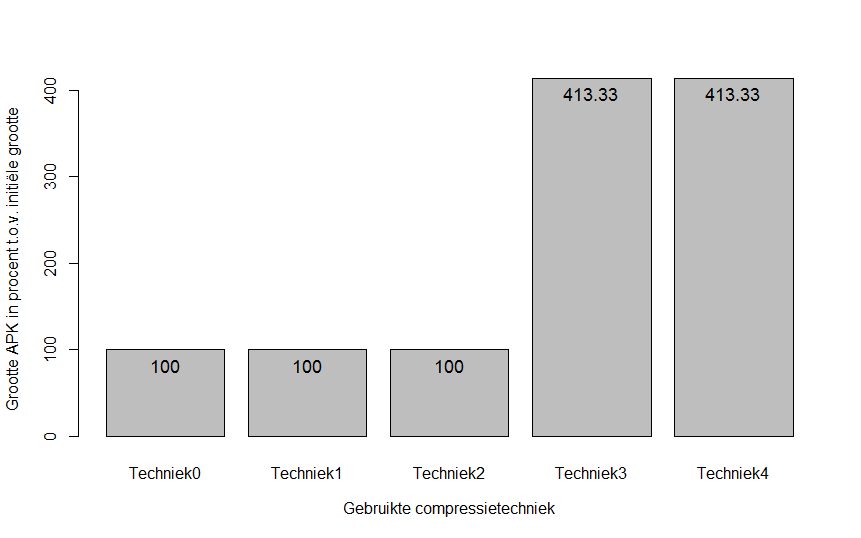
\includegraphics[width=10cm, height=10cm, keepaspectratio]{img/Rplot01}\\[.5cm]
	
\end{figure}

\subsection{Fitness-app}
Bij de tweede applicatie die getest werd, een fitness-app die meer gebruik zal maken van de ingebouwde GPS van het toestel, werden op het vlak van de grootte van de APK geen wijzigingen opgemerkt. De grootte van de APK werd na het toepassen van elke compressietechniek geanalyseerd, maar deze bleef op hetzelfde niveau. Bij het geheugengebruik werd een minieme verandering waargenomen na het toepassen van de 2e techniek, het comprimeren van de afbeeldingen. Het geheugengebruik lag 0.01MB lager na het toepassen van deze techniek. De overige technieken hadden geen invloed op het geheugengebruik. Het CPU-gebruik bleef constant na het toepassen van de verschillende technieken.
\begin{figure}[H]
	\centering
	\caption{\textit{Resultaten verschillende compressietechnieken op APK-grootte fitness-app}}
	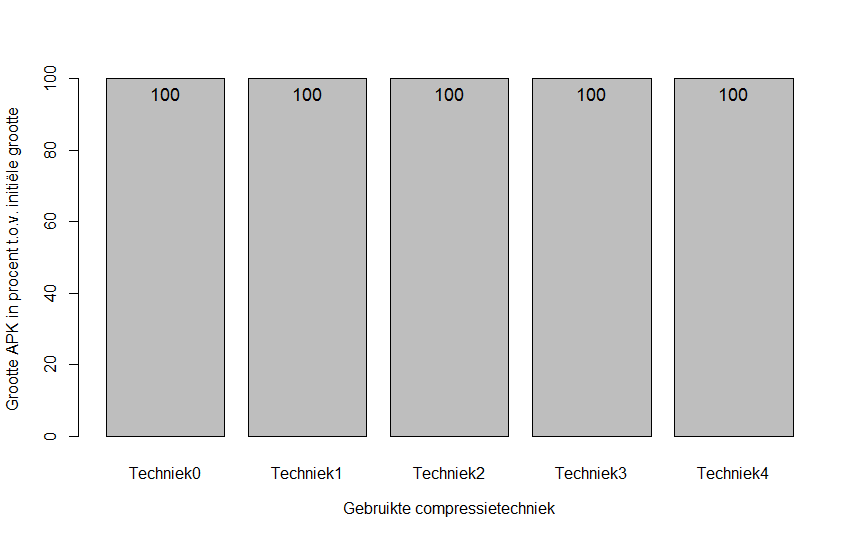
\includegraphics[width=10cm, height=10cm, keepaspectratio]{img/Rplot02}\\[.5cm]
	
\end{figure}
\subsection{CPU-intensieve app}
Bij de derde en laatste applicatie die getest werd, een timer-app die de CPU intensiever gebruikt, werden op het vlak van de grootte van de APK geen wijzigingen opgemerkt. De grootte van de APK werd na het toepassen van elke compressietechniek geanalyseerd, maar deze bleef op hetzelfde niveau. Bij het geheugengebruik werd een verandering van 0.03MB meer geheugen waargenomen na het toepassen van de eerste techniek, het verwijderen van ongebruikte resources. Na het toepassen van de tweede techniek werd er nog een extra toevoeging van 0.01 gebruikt geheugen genoteerd. Het CPU-gebruik was constant na het toepassen van de verschillende technieken.
\begin{figure}[H]
	\centering
	\caption{\textit{Resultaten verschillende compressietechnieken op APK-grootte CPU-intensieve app}}
	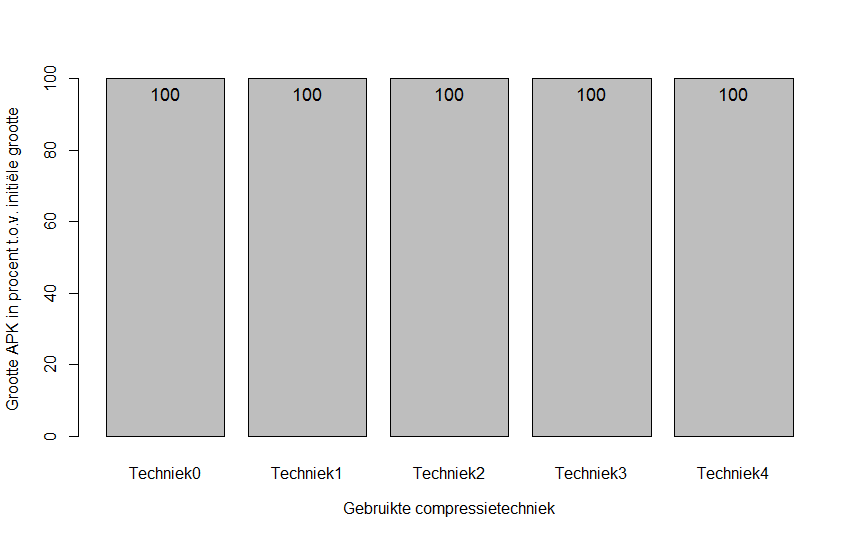
\includegraphics[width=10cm, height=10cm, keepaspectratio]{img/Rplot02}\\[.5cm]
	
\end{figure}

\section{Invloed compressie op prestaties apps}
\label{sec:invloedcompressie}
\subsection{Foto-app}
\subsubsection{Geheugengebruik}
\begin{figure}[H]
	\centering
	\caption{\textit{Resultaten verschillende compressietechnieken op geheugengebruik foto-app}}
	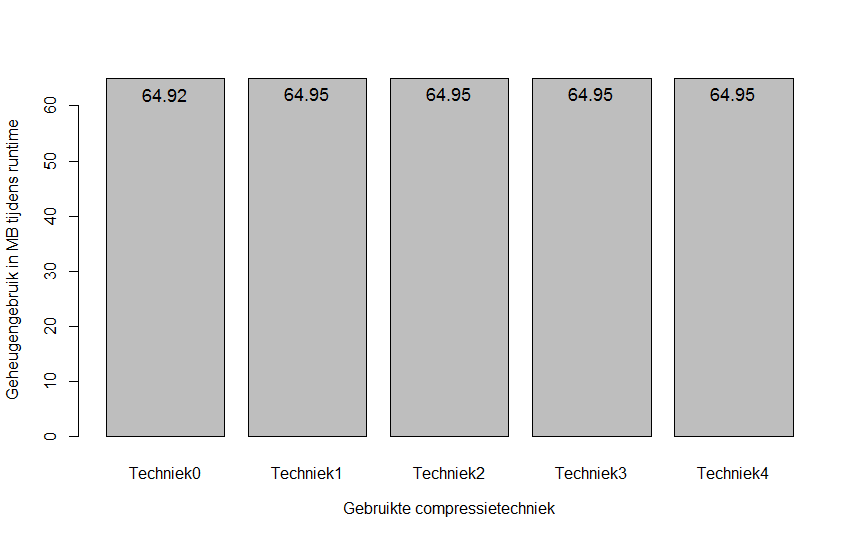
\includegraphics[width=10cm, height=10cm, keepaspectratio]{img/Rplot03}\\[.5cm]
	
\end{figure}
\subsubsection{CPU-gebruik}
\begin{figure}[H]
	\centering
	\caption{\textit{Resultaten verschillende compressietechnieken op CPU-gebruik foto-app}}
	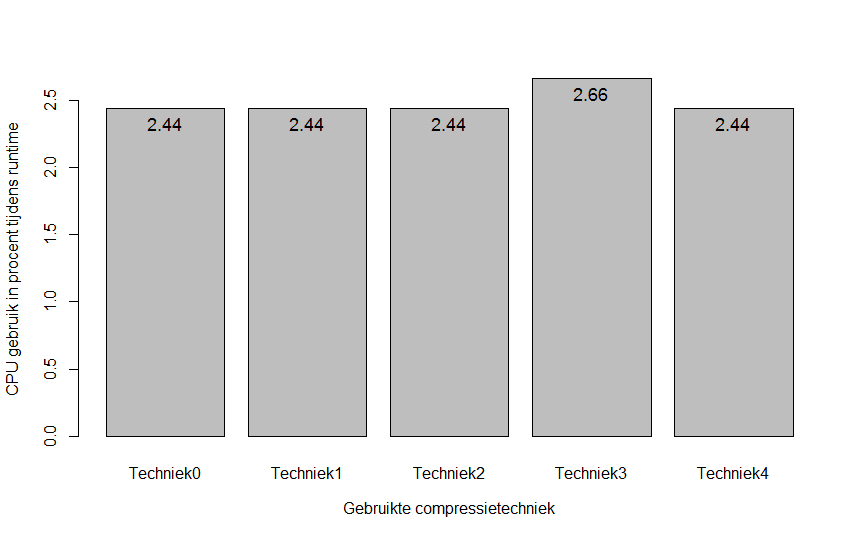
\includegraphics[width=10cm, height=10cm, keepaspectratio]{img/app1cpu}\\[.5cm]
	
\end{figure}
\subsection{Fitness-app}
\subsubsection{Geheugengebruik}
\begin{figure}[H]
	\centering
	\caption{\textit{Resultaten verschillende compressietechnieken op geheugengebruik fitness-app}}
	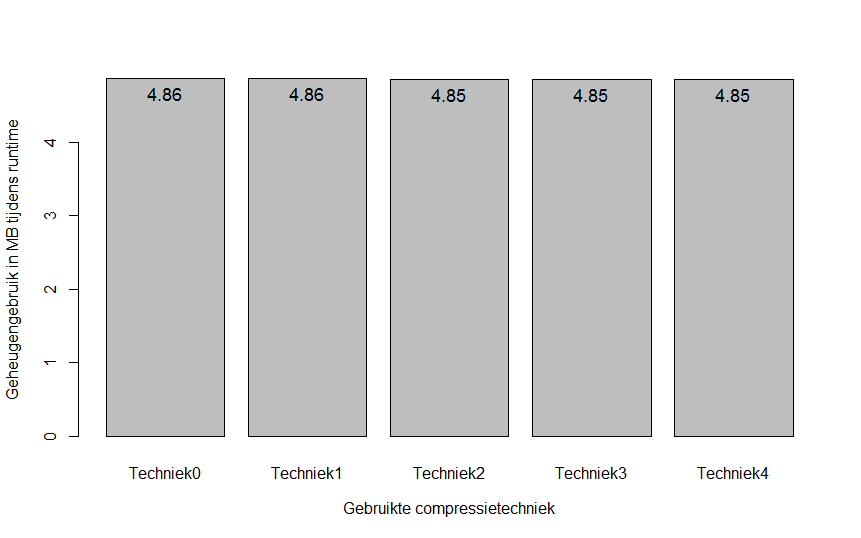
\includegraphics[width=10cm, height=10cm, keepaspectratio]{img/app2geheugen}\\[.5cm]
	
\end{figure}
\subsubsection{CPU-gebruik}
\begin{figure}[H]
	\centering
	\caption{\textit{Resultaten verschillende compressietechnieken op CPU-gebruik fitness-app}}
	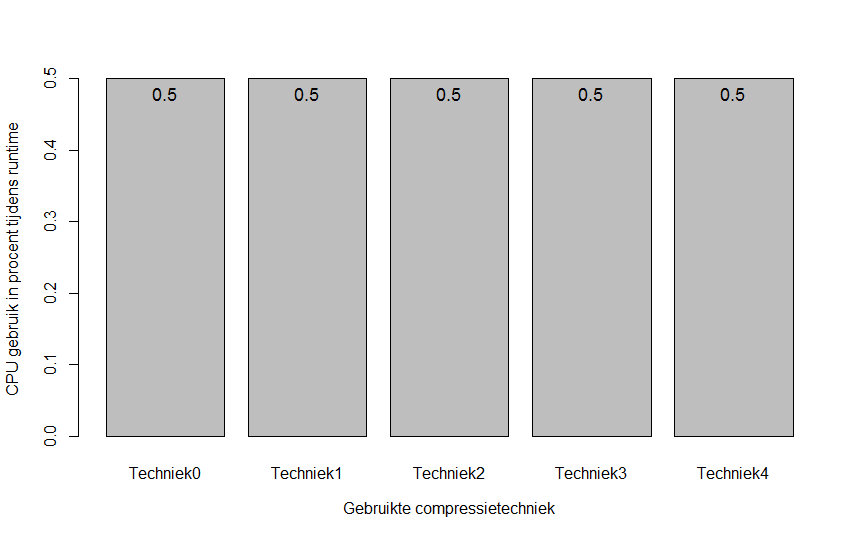
\includegraphics[width=10cm, height=10cm, keepaspectratio]{img/app2cpu}\\[.5cm]
	
\end{figure}
\subsection{CPU-intensieve app}
\subsubsection{Geheugengebruik}
\begin{figure}[H]
	\centering
	\caption{\textit{Resultaten verschillende compressietechnieken op geheugengebruik CPU-intensieve app}}
	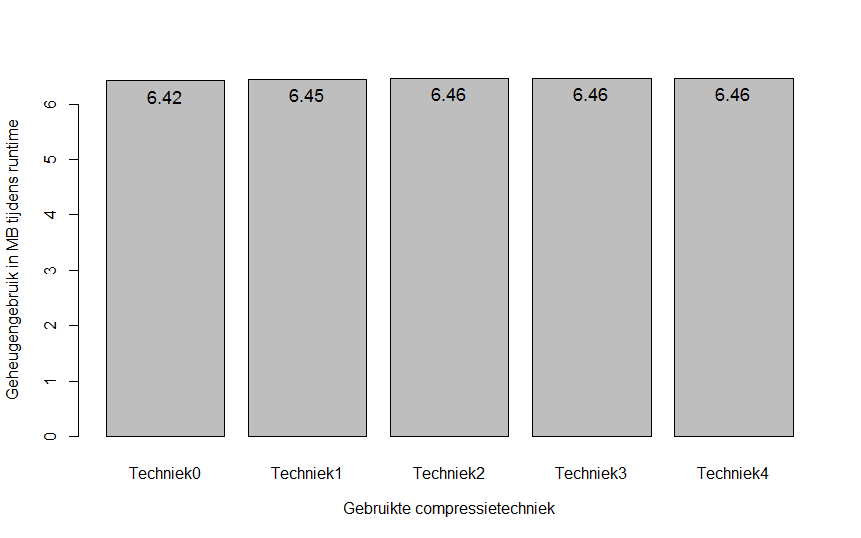
\includegraphics[width=10cm, height=10cm, keepaspectratio]{img/app3geheugen}\\[.5cm]
	
\end{figure}
\subsubsection{CPU-gebruik}
\begin{figure}[H]
	\centering
	\caption{\textit{Resultaten verschillende compressietechnieken op CPU-gebruik CPU-intensieve app}}
	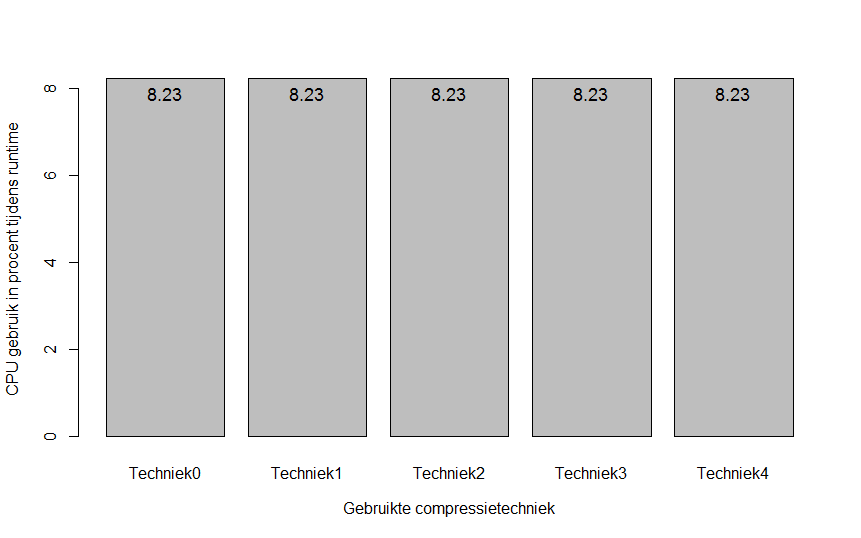
\includegraphics[width=10cm, height=10cm, keepaspectratio]{img/app3cpu}\\[.5cm]
	
\end{figure}

 \section{Testresultaten framework Brian Pinsard}
\label{sec:invloedcompressie}